%%%%%%%%%%%%%%%%%%%%%%%%%%%%%%%%%%%%%%%%%
%Bert Text Abstractive Summarization
% LaTeX Template
% Version 1.4 (15/5/16)
%
% This template has been downloaded from:
% http://www.LaTeXTemplates.com
%
% Original author:
% Frits Wenneker (http://www.howtotex.com) with extensive modifications by
% Vel (vel@LaTeXTemplates.com) and Shane (shanepanter@boisestate.edu)
%
% License:
% CC BY-NC-SA 3.0 (http://creativecommons.org/licenses/by-nc-sa/3.0/)
%
%%%%%%%%%%%%%%%%%%%%%%%%%%%%%%%%%%%%%%%%%

%----------------------------------------------------------------------------------------
%	PACKAGES AND OTHER DOCUMENT CONFIGURATIONS
%----------------------------------------------------------------------------------------
\documentclass[twoside,twocolumn]{article}
\usepackage{biblatex}
\addbibresource{mybib.bib} % with extension

%\usepackage{blindtext} % Package to generate dummy text throughout this template 

\usepackage[sc]{mathpazo} % Use the Palatino font
\usepackage[T1]{fontenc} % Use 8-bit encoding that has 256 glyphs
\linespread{1.05} % Line spacing - Palatino needs more space between lines
\usepackage{microtype} % Slightly tweak font spacing for aesthetics

\usepackage[english]{babel} % Language hyphenation and typographical rules

\usepackage[hmarginratio=1:1,top=32mm,columnsep=20pt]{geometry} % Document margins
\usepackage[hang, small,labelfont=bf,up,textfont=it,up]{caption} % Custom captions under/above floats in tables or figures
\usepackage{booktabs} % Horizontal rules in tables

\usepackage{lettrine} % The lettrine is the first enlarged letter at the beginning of the text

\usepackage{enumitem} % Customized lists
\setlist[itemize]{noitemsep} % Make itemize lists more compact

\usepackage{abstract} % Allows abstract customization
\usepackage{graphicx}
\graphicspath{ {./images/} }
\renewcommand{\abstractnamefont}{\normalfont\bfseries} % Set the "Abstract" text to bold
\renewcommand{\abstracttextfont}{\normalfont\small\itshape} % Set the abstract itself to small italic text

\usepackage{titlesec} % Allows customization of titles
\renewcommand\thesection{\Roman{section}} % Roman numerals for the sections
\renewcommand\thesubsection{\roman{subsection}} % roman numerals for subsections
\titleformat{\section}[block]{\large\scshape\centering}{\thesection.}{1em}{} % Change the look of the section titles
\titleformat{\subsection}[block]{\large}{\thesubsection.}{1em}{} % Change the look of the section titles

\usepackage{fancyhdr} % Headers and footers
\pagestyle{fancy} % All pages have headers and footers
\fancyhead{} % Blank out the default header
\fancyfoot{} % Blank out the default footer
\fancyhead[C]{Bert-Text Abstractive Summarization $\bullet$ April 2021} % Custom header text
\fancyfoot[RO,LE]{\thepage} % Custom footer text

\usepackage{titling} % Customizing the title section

\usepackage{hyperref} % For hyperlinks in the PDF

\usepackage{biblatex}

\usepackage{graphicx}
\graphicspath{ {./images/} }

\usepackage{tablefootnote} % Add a table footnote

%Includes "References" in the table of contents
\usepackage[nottoc]{tocbibind}
%----------------------------------------------------------------------------------------
%	TITLE SECTION
%----------------------------------------------------------------------------------------

\setlength{\droptitle}{-4\baselineskip} % Move the title up

\pretitle{\begin{center}\Huge\bfseries} % Article title formatting
\posttitle{\end{center}} % Article title closing formatting
\title{Bert-Text Abstractive Summarization} % Article title
\author{%
\textsc{Josh Coward}\\[1ex] % Your name
\normalsize Boise State University \\ % Your institution
\normalsize \href{mailto:joshcoward@u.boisestate.edu}{joshcoward@u.boisestate.edu} % Your email address
\and % Uncomment if 2 authors are required, duplicate these 4 lines if more
\textsc{Ryan Pacheco}\\[1ex] % Second author's name
\normalsize Boise State University \\ % Second author's institution
\normalsize \href{mailto:ryanpacheco413@u.boisestate.edu}{ryanpacheco413@u.boisestate.edu} % Second author's email address
\and % Uncomment if 2 authors are required, duplicate these 4 lines if more
\textsc{Sajia Zafreen}\\[1ex] % Third author's name
\normalsize Boise State University \\ % Third author's institution
\normalsize \href{mailto:sajiazafreen@u.boisestate.edu}{sajiazafreen@u.boisestate.edu} % Third author's email address
}
\date{\today} % Leave empty to omit a date
\renewcommand{\maketitlehookd}{%
\begin{abstract}
\noindent 
Text summarization is a process/technique to shorten an extended text such as books, news articles, blog posts, research papers, emails, and tweets in a coherent, fluent summary. It is one of the Natural Language Processing applications, which significantly impacts our lives with a spiking demand every day. With growing digital media and publishing, text summarization helps with deciding on whether an article/ document/ book is valuable or not. With the availability of textual data, it has become easier to train a model for text summarization. This paper discusses Text Abstractive Summarization using Bert to create a model that produces results comparable to Google's massive Pegasus model they developed and released back in June of 2020. We used the English language for our project as it's a language we can speak and understand. We also used the datasets to train our model consist of only English entries. We have used the CNN/Daily Main, SAMSum Corpus, and BillSum Corpus as our datasets.   
\end{abstract}
}

%----------------------------------------------------------------------------------------

\begin{document}

% Print the title
\maketitle


%----------------------------------------------------------------------------------------
%	ARTICLE CONTENTS
%----------------------------------------------------------------------------------------

\section{Introduction}
\lettrine[nindent=0em,lines=3]

Text Summarization summaries extended text while keeping coherent context. The increasing amount of unstructured data needs to be extracted in relevant summaries. There are different types of text summarization: Extractive and Abstractive. Extractive summarization generates a summary by selecting salient sentences or phrases from the source text, while abstractive methods paraphrase and restructure sentences to compose the summary. We focus on abstractive summarization in our work. There are many abstractive approaches based on a sequence-to-sequence model with a copy mechanism. However, some there are issues with these abstractive methods are: 1) because these methods use a left-context decoder while predicting each word, these methods do not have complete context. 2) as they do not use pre-trained contextualized language models on the decoder, the decoded does learn summary representation, context interactions, and language modeling together. 
BERT, which stands for Bidirectional Encoder Representations from Transformation, is designed to pre-train deep bidirectional representations from the unlabeled text by jointly conditioning both left and right context in all layers. As a result, the pre-trained BERT model can be fine-tuned with just one additional output layer to create state-of-the-art models for a wide range of tasks, such as question answering and language inference, without substantial task-specific architecture modifications.\par
BERT is conceptually simple and empirically powerful. It obtains new state-of-the-art results on eleven natural language processing tasks, including pushing the GLUE score to 80.5\% (7.7\% point absolute improvement), MultiNLI accuracy to 86.7\% (4.6\% absolute improvement), SQuAD v1.1 question answering Test F1 to 93.2 (1.5 points absolute improvement) and SQuAD v2.0 Test F1 to 83.1 (5.1 points absolute improvement).\footnote{See "Computation and Language", arXiv:1810.04805 }. \par
Bert has been very successful in textual entailment, name entity recognition, and machine reading comprehension. We have used the Bert-base-uncased pre-trained model for both the encoder and decoder, with the goal in mind of creating a model that resembles to Google's massive Pegasus model.

%------------------------------------------------

\section{Background}



%------------------------------------------------

\subsection{Works Cited}
We have used \cite{aksenov2020abstractive}, \cite{zhang2019pretraining} as reference. In the \cite{aksenov2020abstractive} paper, the text summarization model is based on the Transformer architecture. The architecture adopts the original model of Vaswami et al. (2017). On top of the decoder, they used a Pointer-Generator to increase the extractive capabilities of the network. In Paper \cite{zhang2019pretraining}, proposed 1. A natural language generation model based on BERT, making good use of the pre-trained language model in the encoder and decoder process, and the model can be trained end-to-end without handcrafted features. 2. A design a two-stage decoder process. In this architecture, our model can generate each word of the summary considering both sides’ context information. 3. To conduct experiments on the benchmark datasets CNN/Daily Mail and New York Times. Our model achieves a 33.33 average of ROUGE-1, ROUGE-2 and ROUGE-L on the CNN/Daily Mail, which is state-of-the-art. On the New York Times dataset, our model achieves about 5.6\% relative improvement over ROUGE-1. 
Our work doesn't differ much from the papers we referenced here \cite{aksenov2020abstractive}, \cite{zhang2019pretraining}. As BERT can't process sequences with more than 512 tokens, to deal with that our model is using overlapping subsection text of length 512 words and generating summaries for each of the individual subsections. In the end, a final summary across all those summaries. In the case of summaries, we didn't use a pre-trained summary model until the end.


%------------------------------------------------

\subsection{Datasets}

Our project used three datasets: \textbf{1) CNN/Dailymail, 2) SAMSum corpus, and 3) Billum corpus}. There are different datasets for text summarization. We tried to find datasets with "gold" summaries to compare our generated summaries with the "gold" summaries for our approach.\par 

The \textbf{CNN/Dailymail} is an English-language dataset containing just over 300k unique news articles written by journalists at CNN and the Daily Mail. We have used version 3.0.0, which can be used to train both abstractive and extractive summarization.\par
The data consists of news articles and highlight sentences. In the question answering setting of the data, the articles are used as the context and entities are hidden one at a time in the highlight sentences, producing Cloze style questions where the goal of the model is to correctly guess which entity in the context has been hidden in the highlight. In the summarization setting, the highlight sentences are concatenated to form a summary of the article. The CNN articles were written between April 2007 and April 2015. The Daily Mail articles were written between June 2010 and April 2015.
The model performance is measured by how high the output summary's ROUGE score for a given article is compared to the highlight written by the original article author. Zhong et al. (2020) report a ROUGE-1 score of 44.41 when testing a model trained for extractive summarization. See the Papers With Code leaderboard for more models.\footnote{See "Get To The Point: Summarization with Pointer-Generator Networks", https://www.aclweb.org/anthology/P17-1099}. There is a string for the article for each instance, a string for the highlights, and a string for the id.  The train set has 287,113, the validation set has 13,368, and the Test set has 11,490 instances in Split.

The \textbf{SAMSum} dataset contains about 16k messenger-like conversations with summaries. Conversations were created and written down by linguists fluent in English. The dataset reflects the proportion of topics of real-life messenger conversations.  It has 16369 conversations distributed uniformly into 4 groups. Each instance contains an id string, a summary string, and a dialogue string.  The train set has 14,732, the validation set has 818, and the test set has 819 instances in Split.  The summaries are annotated and assume they should 1) be short, 2) extract important pieces of information, 3)include names of interlocutors, and 4)be written in the third person. Each dialogue has only one reference of summary.\footnote{See "{SAMS}um Corpus: A Human-annotated Dialogue Dataset for Abstractive Summarization", https://www.aclweb.org/anthology/D19-5409} \par

The \textbf{BillSum} dataset summarizes the state bills of US Congressional and California states. It has several features: 1)text: bill text, 2) summary: summary of the bills, 3)title: title of the bills, 4)text\_len: number of chars in text, 5)sum\_len: number of chars in summary. The data field has a text string, a \cite{aksenov2020abstractive} summary string, and a title string. The train set has 18,949,  the ca\_test set has 1237, and the test set has 3269 instances in Split.\footnote{See "BillSum: A Corpus for Automatic Summarization of US Legislation", 1910.00523}



%------------------------------------------------

\section{Model and Approach}
In the encoding and generation process, the attention mechanism is used to concentrate on the most important positions of text. The learning objective of most sequence-to-sequence models is to minimize the negative log likelihood of the generated sequence as shown in following equation, where y$^*_{t}$ is the t-th ground-truth summary token.

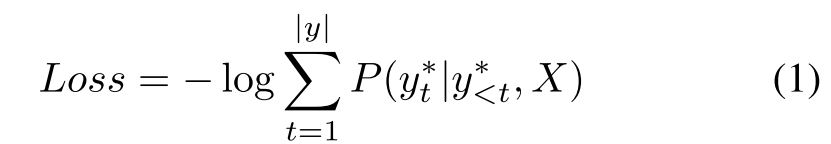
\includegraphics[width=0.45\textwidth,height=0.9\textheight,keepaspectratio]{equal0.JPG}

We used BERT and tried to fine tune it. BERT consists of several layers. In each layer, there is a first multi-head self-attention sub-layer and then a linear sub layer with residual connection. In each self-attention sub-layer the attention scores e$_{ij}$ are first calculated as Eq. (2), (3), in which d$_{e}$ is output dimension, and W$^Q$, W$^K$, W$^V$ are parameter matrices. 

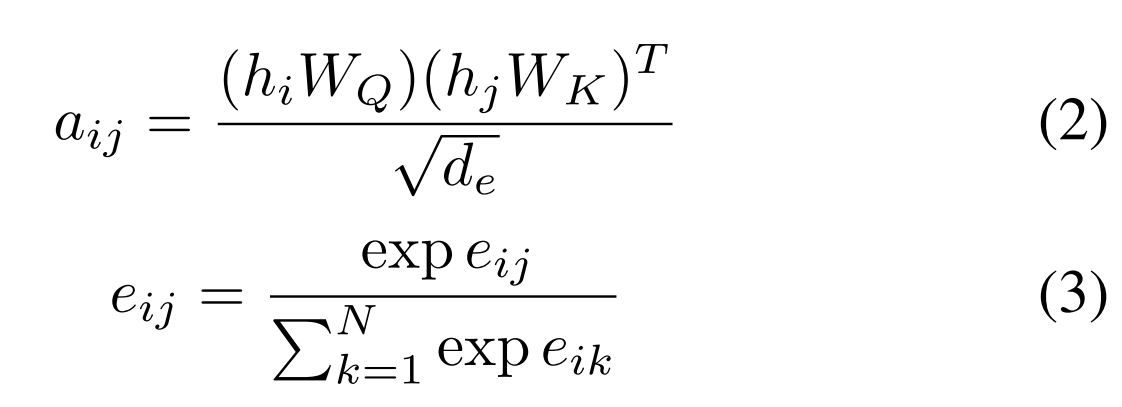
\includegraphics[width=0.45\textwidth,height=0.9\textheight,keepaspectratio]{equa1.JPG}

Then the output is calculated as Eq. (4), which is the weighted sum of previous outputs h added by previous out-put h$_{i}$. The last layer outputs are context encoding of input sequence.

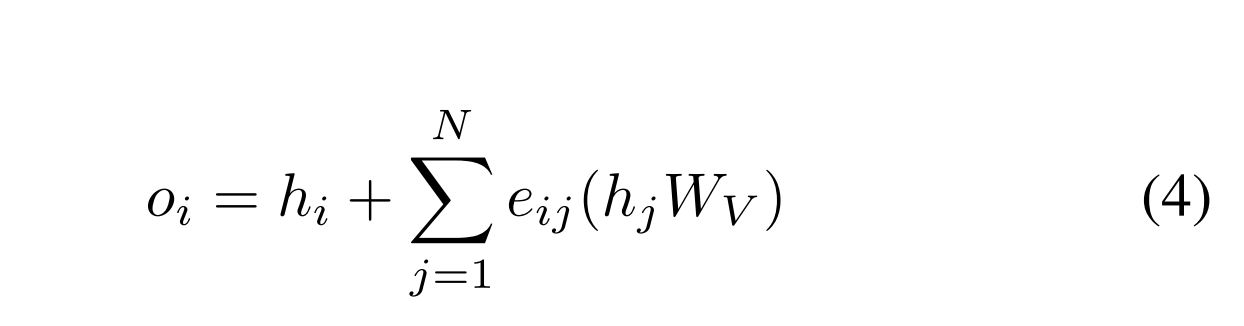
\includegraphics[width=0.45\textwidth,height=0.9\textheight,keepaspectratio]{equa2.JPG}

Despite the wide usage and huge success, there is also a mismatch problem between these pre-trained context encoders and sequence-to-sequence models. The issue is that while using a pre-trained context encoder like BERT, they model token-level representations by conditioning on both direction context. During pre-training, they are fed with complete sequences. However, with a left-context-only decoder, these pre-trained language models will suffer from incomplete and inconsistent context and thus cannot generate good enough context-aware word representations, especially during the inference process.

Based on the sequence-to-sequence framework built on top
of BERT, we first followed the design mentioned in \cite{zhang2019pretraining}, which is a refine decoder at word-level to tackle the two problems described in the above section. We also introduce a discrete objective for the refine decoders to reduce the exposure bias problem.

%------------------------------------------------

\section{Evaluation}
%------------------------------------------------

\section{Implications}
%------------------------------------------------

\section{Results}


%------------------------------------------------

\section{Conclusion}

%------------------------------------------------


%----------------------------------------------------------------------------------------
%	REFERENCE LIST
%----------------------------------------------------------------------------------------

%\section{References}    

%\cite{aksenov2020abstractive}

\printbibliography

  
%----------------------------------------------------------------------------------------

% FOR REFERENCE




\end{document}
